%% Requires compilation with XeLaTeX or LuaLaTeX
\documentclass[compress,10pt,xcolor={table,dvipsnames},t]{beamer}
\usetheme{diapo}
%\usepackage{hyperref}
\usepackage{amsmath}
\usepackage{amssymb}
\usepackage{xcolor}
\usepackage[bottom]{footmisc}
\usepackage{multirow}
\usepackage{setspace}
\usepackage{caption}
\usepackage{array,multirow,makecell}
\usepackage{pifont}
%\usepackage[colorlinks=true]{hyperref}
\usepackage{tikz}
\usepackage{paralist}
\usepackage{appendixnumberbeamer}
\usepackage[backend=biber,style=numeric,sorting=nyt,doi=false,url=false]{biblatex}
\usepackage{etoolbox}
% box colorée dans équation
\usepackage[most]{tcolorbox}
\usepackage{tikz}
\usepackage{soul}
% pour l'indicatrice
\usepackage{dsfont}


\setcellgapes{1pt}
\setlength{\parindent}{0pt}
\makegapedcells
\newcolumntype{R}[1]{>{\raggedleft\arraybackslash }b{#1}}
\newcolumntype{L}[1]{>{\raggedright\arraybackslash }b{#1}}
\newcolumntype{C}[1]{>{\centering\arraybackslash }b{#1}}
\renewcommand*{\bibfont}{\scriptsize}
% Supprimer "In:" pour les articles
\renewbibmacro{in:}{}
% Supprimer les champs d'eprints
\AtEveryBibitem{\clearfield{arxiv}}
\AtEveryBibitem{\clearfield{eprint}}
\AtEveryBibitem{\clearfield{note}}
\AtEveryBibitem{\clearfield{eprintclass}}
\AtEveryBibitem{\clearfield{eprinttype}}
% Supprimer les URL
\ExecuteBibliographyOptions{url=false}
% Charger votre fichier de bibliographie
\addbibresource{biblio.bib}
\useoutertheme[subsection=false]{miniframes}
\makeatletter
\patchcmd{\slideentry}{\advance\beamer@xpos by1\relax}{}{}{}
\def\beamer@subsectionentry#1#2#3#4#5{\advance\beamer@xpos by1\relax}%
\makeatother
\setbeamercolor*{mini frame}{fg=bulles,bg=bulles}
\hypersetup{
	colorlinks=true,
	urlcolor=blue,
	citecolor=blue,
	linkcolor=title,
}

\title[PhiFEM]{Mesh-based methods and physically informed learning}
\subtitle{Macaron/Tonus retreat presentation}
\authors[LECOURTIER Frédérique]
\supervisors[DUPREZ Michel, FRANCK Emmanuel, LLERAS Vanessa]
\date{February 6-7, 2024}

\allowbreak

% u_chapeau (chapeau en couleur)
\usepackage{accents}
\newcommand{\uchapeau}[1]{\accentset{\textcolor{red}{\wedge}}{#1}}
\newcommand{\refappendix}[1]{\tikz[baseline=(char.base)]{\node[framednumber] (char) {\hyperlink{#1}{\small \textcolor{white}{Appendix \ref*{#1}}}};}}

\definecolor{appendix}{RGB}{180, 189, 138}
\tikzset{
	framednumber/.style={
		draw=appendix,% Couleur de la bordure
		fill=appendix, % Couleur de fond
		rounded corners, % Coins arrondis
		inner sep=2pt,  % Espace intérieur
	}
}

% numérotation et label des appendix
\newcounter{appendixframenumber}
\setcounter{appendixframenumber}{1}

\makeatletter
\newcommand{\labelappendixframe}[1]{%
	\protected@write\@auxout{}{%
		\string\newlabel{#1}{{\theappendixframenumber}{\thepage}}%
	}%
	\hypertarget{#1}{}
}	
\makeatother

%\newenvironment{appendixframe}[2][]{%
%	\begin{frame}[#1]{\appendixname~\theappendixframenumber~: #2}%
%	}{%
%	\end{frame}
%	\addtocounter{appendixframenumber}{1}
%}

\begin{document}
	\nocite{*}
	
	\renewcommand{\inserttotalframenumber}{\pageref{lastslide}}
	
	{\setbeamertemplate{footline}{} 
		\begin{frame}
			\maketitle
		\end{frame}
	}
	\addtocounter{framenumber}{-1} 
	
	\AtBeginSection[]{
		{\setbeamertemplate{footline}{}
			\begin{frame}
				\vfill
				\centering
				\begin{beamercolorbox}[sep=5pt,shadow=true,rounded=true]{subtitle}
					\usebeamerfont{title}\insertsectionhead\par%
				\end{beamercolorbox}
				%\tableofcontents[sectionstyle=hide,subsectionstyle=show]
				
				%subsectionstyle=⟨style for current subsection⟩/⟨style for other subsections in current section⟩/⟨style for subsections in other sections⟩
				\tableofcontents[sectionstyle=hide,subsectionstyle=show/show/hide]
				\vfill
			\end{frame}
		}
		\addtocounter{framenumber}{-1} 
	}
	
	\AtBeginSubsection[]{
		{\setbeamertemplate{footline}{}
			\begin{frame}
				\vfill
				\centering
				\begin{beamercolorbox}[sep=5pt,shadow=true,rounded=true]{subtitle}
					\usebeamerfont{title}\insertsectionhead\par%
				\end{beamercolorbox}
				\tableofcontents[sectionstyle=hide,subsectionstyle=show/shaded/hide]
				\vfill
			\end{frame}
		}
		\addtocounter{framenumber}{-1} 
	}
	
	% \begin{frame}{Test anmiation}
		%     \begin{center}
			%         \begin{animateinline}[autoplay,loop,controls]{3} 
				%     		% \multiframe{11}{rPos=0+0.1}{ 
					%     		% 	\begin{tikzpicture}
						%     		% 		\draw[start segment=\rPos,black!70, line width=2.5] (0,0) -- (1,0) -- (1,1) -- (0,1) --cycle ;
						%      	% 		\end{tikzpicture} 
					%     		% } 
				%         \animate<1-2>
				%         \multiframe{2}{rX=1+1}{
					%         \begin{center}
						%           \includegraphics[width=0.2\textwidth]{images/image\rX.png}
						%         \end{center}
					%         }
				%     	\end{animateinline} 
			%     \end{center}
		% \end{frame}
	
	\section{Introduction}
	\begin{frame}{Scientific context}
    \textbf{Context :} Create real-time digital twins of an organ (such as the liver).

    \textbf{$\phi$-FEM Method :} New fictitious domain finite element method.

    \begin{enumerate}[\ding{217}]
        \item domain given by a level-set function $\Rightarrow$ don't require a mesh fitting the boundary 
        \item allow to work on complex geometries 
        \item ensure geometric quality 
        % \item Cartesian grid adapted for neural networks
    \end{enumerate}
    
    \begin{center}
        \pgfimage[width=0.65\linewidth]{images/intro/context_geometry.png}
    \end{center}	

    \textit{Practical case:} Real-time simulation, shape optimization...
\end{frame}

\begin{frame}{Objective}
    \textbf{Current Objective :} Develop hybrid finite element / neural network methods.

	\begin{center}
		\begin{tcolorbox}[
			colback=white, % Couleur de fond de la boîte
			colframe=other, % Couleur du cadre de la boîte
			arc=2mm, % Rayon de l'arrondi des coins
			boxrule=0.5pt, % Épaisseur du cadre de la boîte
			breakable, enhanced jigsaw,
			width=0.8\linewidth
			]
			
			\textbf{OFFLINE :}
			
			\begin{figure}[htb]
				\centering
				\resizebox{\textwidth}{!}{%
					\begin{tikzpicture}
						\node at (0,0.8) {Several Geometries};
						\node[draw=none, inner sep=0pt] at (0,0) {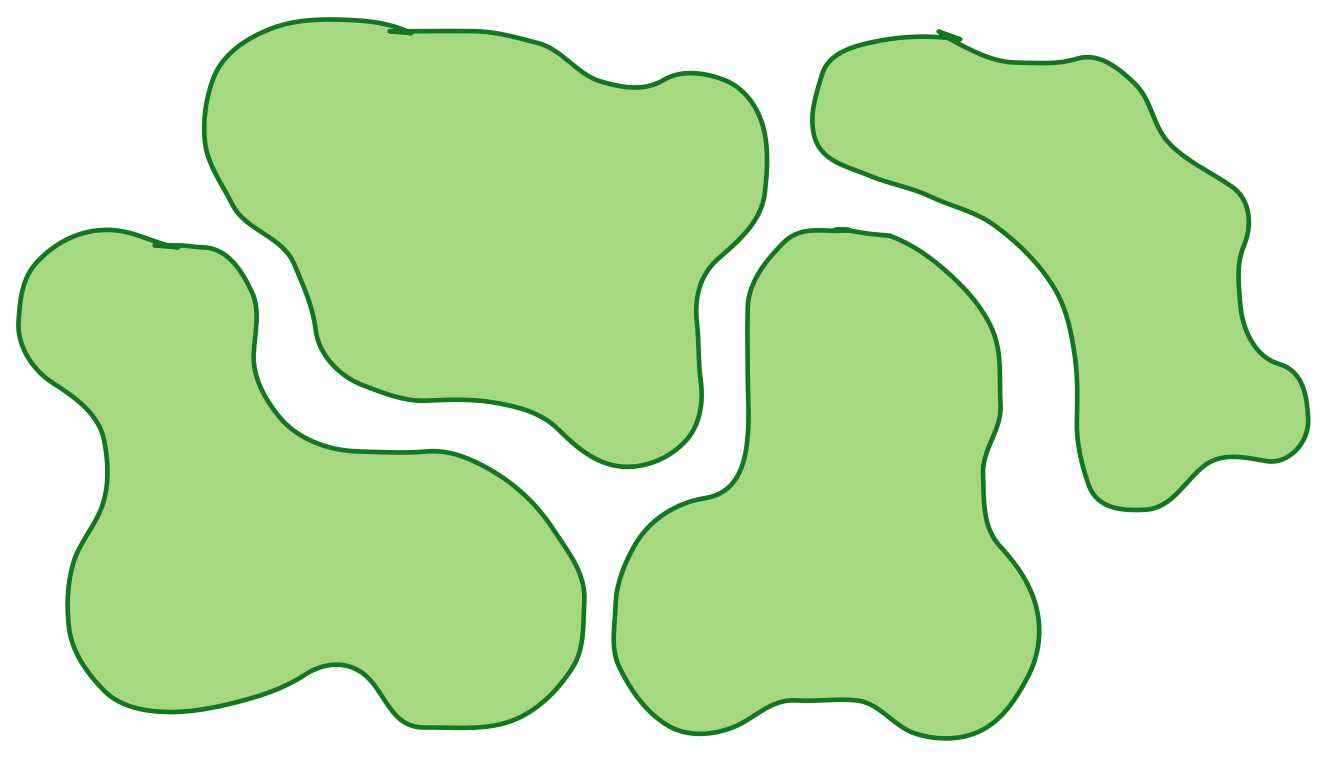
\includegraphics[width=2cm]{images/intro/objective_geom.png}};
						\node[title,font=\Large] at (1.6,0.1) {+};
						\node at (3.5,0.8) {Several Functions};
						\node[draw=none, inner sep=0pt] at (3.5,0) {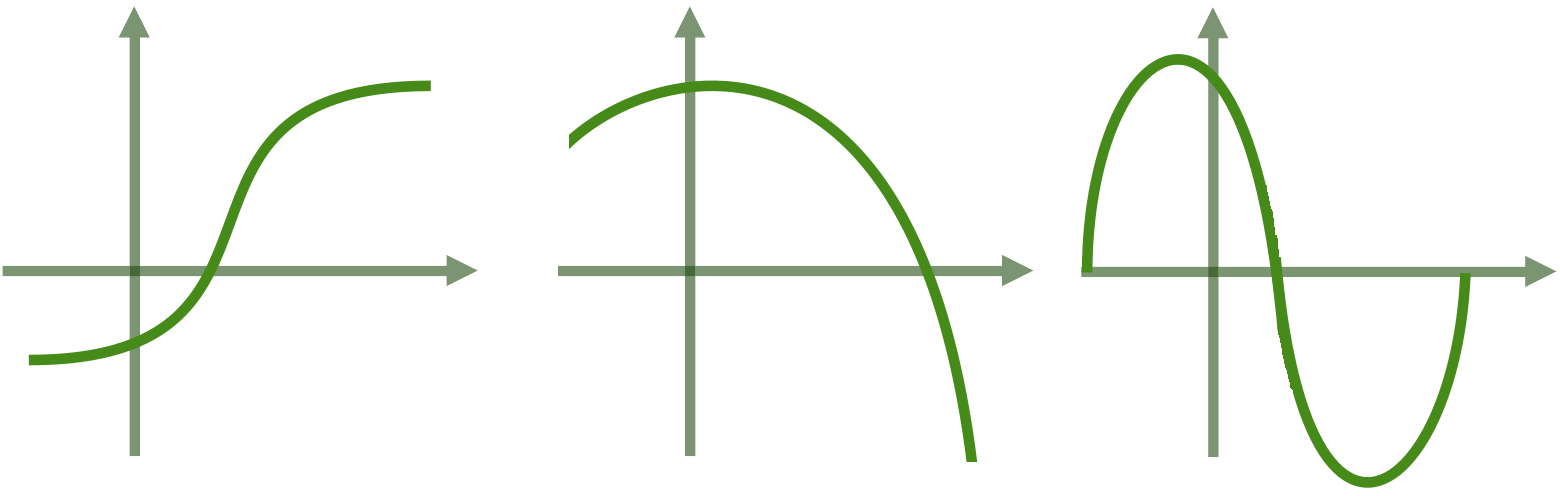
\includegraphics[width=3cm]{images/intro/objective_fct.png}};
						
						% Ajouter une flèche entre les deux rectangles
						\draw[->, title, line width=1.5pt] (5.5,0.1) -- (6.5,0.1);
						%		
						\node at (8,0.8) {Train a PINNs};
						\node[draw=none, inner sep=0pt] at (8,-0.1) {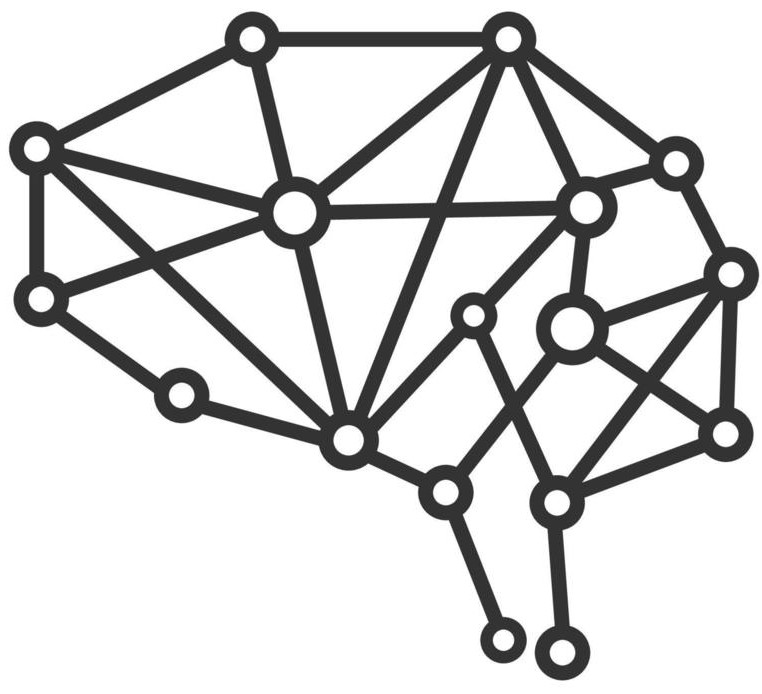
\includegraphics[width=1.5cm]{images/intro/objective_pinns.jpg}};				
					\end{tikzpicture}
				}%
			\end{figure}
			
			\textbf{ONLINE :}
			
			\vspace{-25pt}
			
			\begin{figure}[htb]
				\centering
				\resizebox{\textwidth}{!}{%
					\begin{tikzpicture}
						\node at (0,0.8) {1 Geometry - 1 Function};
						\node[draw=none, inner sep=0pt] at (0,0) {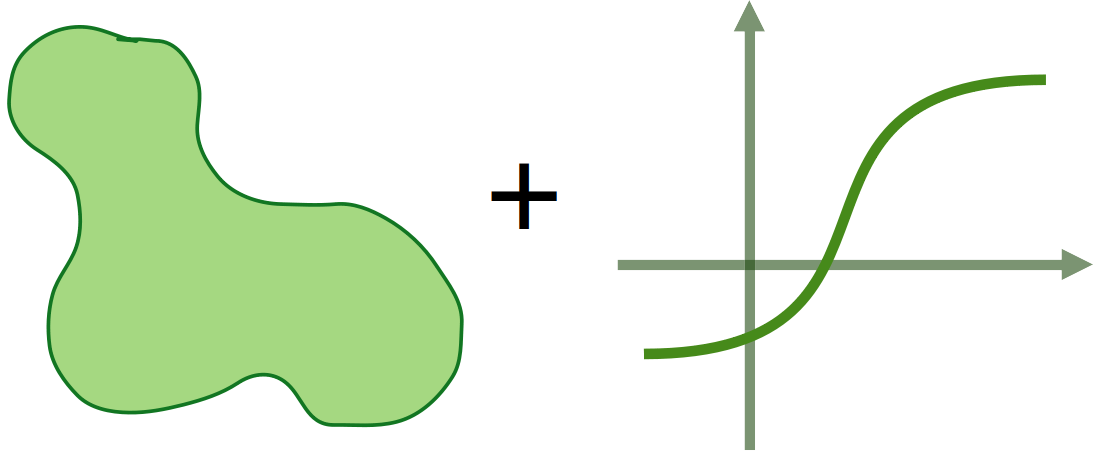
\includegraphics[width=2cm]{images/intro/objective_onegeom_onefct.png}};
						%		\node[title,font=\Large] at (1.6,0.1) {+};
						%		\node at (3.5,0.8) {Several Functions};
						%		\node[draw=none, inner sep=0pt] at (3.5,0) {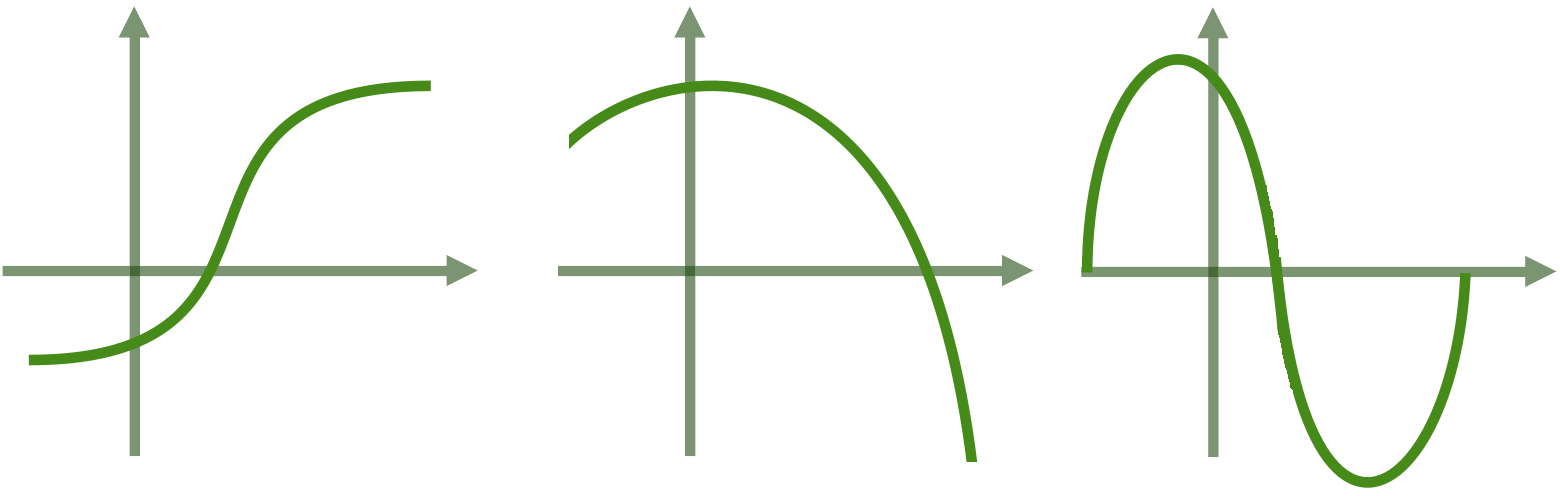
\includegraphics[width=3cm]{images/intro/objective_fct.png}};
						
						\draw[->, title, line width=1.5pt] (2,0.1) -- (3,0.1);
						
						\node[align=center] at (4,1) {Get PINNs \\ prediction};
						\node[draw=none, inner sep=0pt] at (4,-0.1) {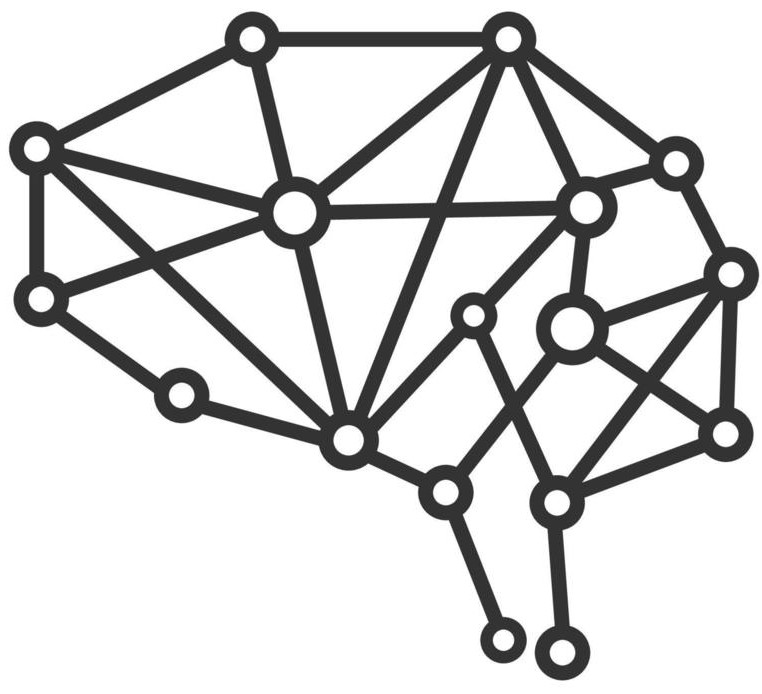
\includegraphics[width=1.5cm]{images/intro/objective_pinns.jpg}};
						
						% Ajouter une flèche entre les deux rectangles
						\draw[->, title, line width=1.5pt] (5.5,0.1) -- (6.5,0.1);
						%		
						\node[align=center] at (8,1) {Correct prediction \\ with $\phi$-FEM};
						\node[draw=none, inner sep=0pt] at (8,-0.1) {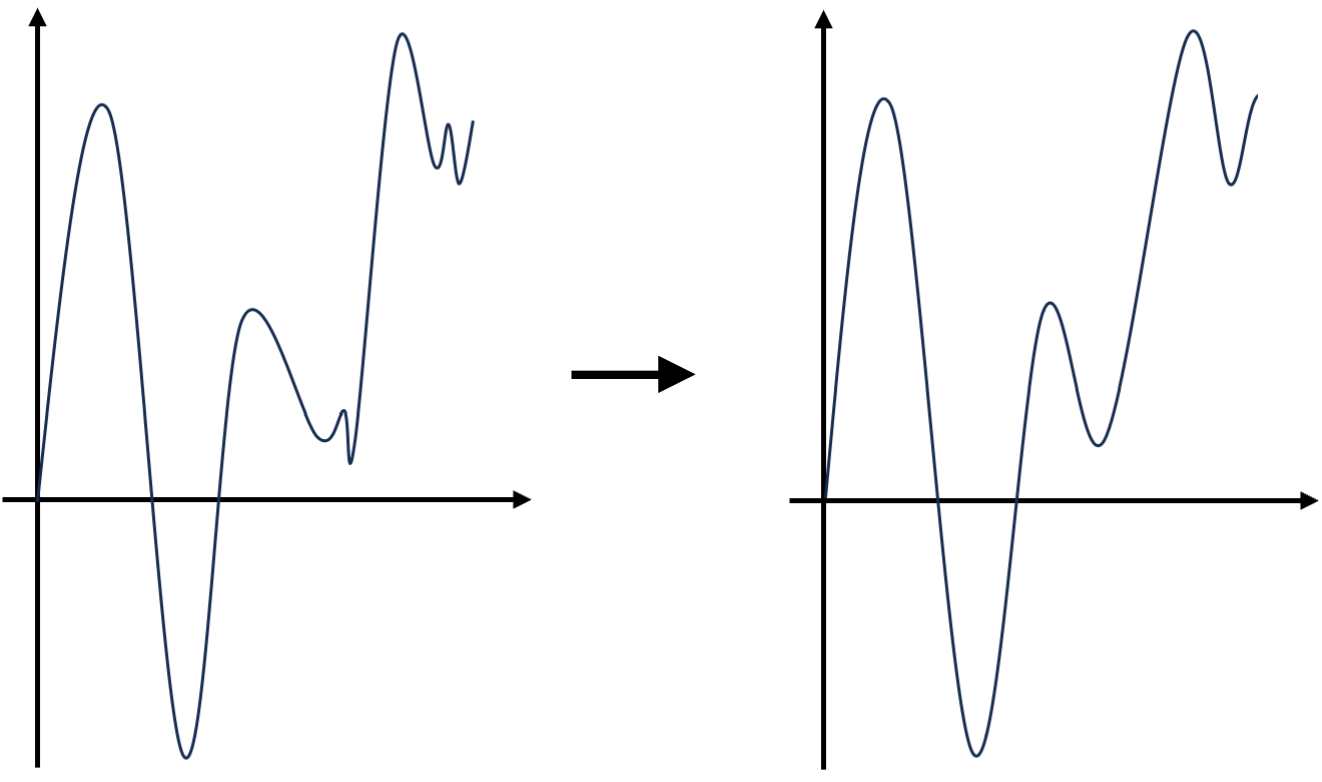
\includegraphics[width=2.5cm]{images/intro/objective_corr.png}};		
					\end{tikzpicture}
				}%
			\end{figure}
		\end{tcolorbox}
	\end{center}

    \textbf{Evolution :}

    \small
    % \setstretch{0.5}
    \begin{itemize}
        \item Geometry : 2D, simple, fixed (as circle, ellipse..) $ \; \rightarrow \;$ 3D / complex / variable
        \item PDE : simple, static (Poisson problem) $\; \rightarrow \;$ complex / dynamic (elasticity, hyper-elasticity)
        \item Neural Network : simple and defined everywhere (PINNs) $\; \rightarrow \;$ Neural Operator
    \end{itemize}
\end{frame}

\begin{frame}{Problem considered}
    \textbf{Elliptic problem with Dirichlet conditions :} \\
    Find $u : \Omega \rightarrow \mathbb{R}^d (d=1,2,3)$ such that
    \begin{equation}
    	\left\{\begin{aligned}
    		&L(u)=-\nabla \cdot (A(x) \nabla u(x)) + c(x)u(x) = f(x) \quad \text{in } \Omega, \\
    		&u(x) = g(x) \quad \text{on } \partial \Omega
    	\end{aligned}\right. \label{edp}
    \end{equation}
	with $A$ a definite positive coercivity condition and $c$ a scalar. We consider $\Delta$ the Laplace operator, $\Omega$ a smooth bounded open set and $\Gamma$ its boundary. 
    
    \textbf{Weak formulation :}
    \begin{equation*}
    	\text{Find } u\in V \text{ such that } a(u, v) = l (v) \forall v\in V
    \end{equation*}
    
    with
    \begin{align*}
    	a(u,v)&=\int_{\Omega} (A(x)\nabla u(x)) \cdot \nabla v(x) + c(x)u(x)v(x) \, dx \\
    	l(v)&=\int_{\Omega} f(x)v(x) \, dx
    \end{align*}
    
    \footnotesize
    \textit{Remark :} For simplicity, we will not consider 1st order terms. 

%    We will define by
%    \begin{equation*}
%        ||u_{ex}-u_{method}||_{0,\Omega}^{(rel)}=\frac{\int_\Omega (u_{ex}-u_{method})^2}{\int_\Omega u_{ex}^2}
%    \end{equation*}
%    the relative error between
%    \begin{itemize}
%        \item $u_{ex}$ : the exact solution  
%        \item $u_{method}$ : the solution obtained by a method \\
%        (can be : FEM or $\phi$-FEM, a correction solver or the prediction of an neural network).
%    \end{itemize}
\end{frame}

\begin{frame}{Numerical methods}
	\textbf{Objective :} Show that the philosophy behind most ofd the methods are the same.
	\begin{center}
		Mesh-based methods \hspace{5pt} // \hspace{5pt} Physically informed learning
	\end{center}
	
	\textbf{Numerical methods :} Discrete an infinite-dimensional problem (unknown = function) and solve it in a finite-dimensional space (unknown = vector).
	\begin{enumerate}[\textbullet]
		\item \textbf{Encoding :} we encode the problem in a finite-dimensional space
		\item \textbf{Approximation :} solve the problem in finite-dimensional space
		\item \textbf{Decoding :} bring the solution back into infinite dimensional space
	\end{enumerate}
	
	\begin{center}
		\begin{tabular}{|c|c|c|}
			\hline
			\textbf{Encoding} & \textbf{Approximation} & \textbf{Decoding} \\
			\hline
			$f \; \rightarrow \theta_f$ & $\theta_f \; \rightarrow \theta_u$ & $\theta_u \; \rightarrow u_\theta$ \\
			\hline
		\end{tabular}
	\end{center}
\end{frame}

	
	\section{Mesh-based methods}
	\subsection{Encoding/Decoding}

\begin{frame}{Encoding/Decoding - FEMs}
	\begin{itemize}[\textbullet]
		\item \textbf{Decoding :} Linear combination of piecewise polynomial function $\varphi_i$.
		\begin{equation*}
			\mathcal{D}_{\theta_u}(x) = \sum_{i=1}^{N}(\theta_u)_i\varphi_i
		\end{equation*}
		$\Rightarrow$ linear decoding $\Rightarrow$ approximation space $V_N$ = vectorial space \\
		$\Rightarrow$ existence and uniqueness of the orthogonal projector
		\item \textbf{Encoding :} Orthogonal projection on vector space $V_N=Vect\{\varphi_1,\dots,\varphi_N\}$.
		\begin{equation*}
			\theta_f=E(f)=M^{-1}b(f)
		\end{equation*}
		with $M_{ij}=\int_\Omega \varphi_i(x)\varphi_j(x)$ and $b_i(f)=\int_\Omega \varphi_i(x)f(x)$. \refappendix{frame:encoding_fems} 
	\end{itemize}
\end{frame}

\subsection{Approximation}

\begin{frame}{Approximation}
	\textbf{Idea :} Project a certain form of the equation onto the vector space $V_N$. \\
	We introduce the residual of the equation defined by
	\begin{equation*}
		R(v) = R_{in}(v)\mathds{1}_{\Omega} + R_{bc}(v)\mathds{1}_{\partial \Omega}
	\end{equation*}
	with 
	\begin{equation*}
		R_{in}(v)=L(v) - f \qquad \text{and} \qquad R_{bc}(v)=v-g
	\end{equation*}
	which respectively define the residues inside $\Omega$ and on the boundary $\partial\Omega$. 
	
	\vspace{10pt}
	
	\textbf{Discretization :} Degrees of freedom problem (which also has a unique solution)
	\begin{center}
		$u=\arg\min_{v\in V_N} J(v) \quad \longrightarrow \quad \theta_u=\arg\min_{\theta\in \mathbb{R}^N} J(\theta) $
	\end{center}
	with $J$ a functional to minimize.
	
	\vspace{10pt}
	
	\textbf{Variants :} Depends on the problem form used for projection.
	
	\begin{center}
		\begin{tabular}{c|c}
			Problem - Energetic form & Problem - Least-square form \\
			Galerkin projection & Galerkin Least-square projection
		\end{tabular}
	\end{center}
\end{frame}

\begin{frame}{Energetic form}
	\textbf{Minimization Problem :}
	\begin{equation}
		u_\theta(x)=\arg\min_{v\in V_N} J(v), \qquad J(v)=J_{in}(v)+J_{bc}(v)\label{minpb_galerkin}
	\end{equation}
	with 
	\begin{equation*}
		J_{in}(v)=\frac{1}{2}\int_\Omega L(v)v - \int_\Omega fv  \qquad \text{et} \qquad J_{bc}(v)=\frac{1}{2}\int_\Omega R_{bc}(v)^2
	\end{equation*}

	\footnotesize	
	\textit{Remark :} This form of the problem is due to the Lax-Milgram theorem as $a$ is symmetrical.
	\normalsize
	
	\footnotesize
	\begin{center}
		\begin{tcolorbox}[
			colback=white, % Couleur de fond de la boîte
			colframe=other, % Couleur du cadre de la boîte
			arc=2mm, % Rayon de l'arrondi des coins
			boxrule=0.5pt, % Épaisseur du cadre de la boîte
			breakable, enhanced jigsaw,
			width=0.8\linewidth
			]
			
			\textbf{Minimization Problem \eqref{minpb_galerkin} $\Leftrightarrow$ PDE \eqref{edp} :}
			
			\centering
			$\nabla_v \; J(v)=R(v) \qquad $ \refappendix{frame:minpb_galerkin} 
			
			\vspace{5pt}
			
			\begin{minipage}{0.1\linewidth}
				\centering
				$u_\theta$ sol \\
				of \eqref{minpb_galerkin}
			\end{minipage} $\Leftrightarrow \; \nabla_{u_\theta} \; J(u_\theta)=0 \; \Leftrightarrow \; \left\{\begin{aligned}
				&R_{in}(u_\theta)=0 \; \text{in} \; \Omega \\
				&u_\theta=g \; \text{on} \; \partial\Omega
			\end{aligned}\right. \; \Leftrightarrow$ \begin{minipage}{0.1\linewidth}
				\centering
				$u_\theta$ sol \\
				of \eqref{edp}
			\end{minipage}
		
			\vspace{5pt}
			
			\begin{minipage}{0.1\linewidth}
				\centering
				\textbf{Min pb}
			\end{minipage} \; \hspace{150pt} \; \begin{minipage}{0.1\linewidth}
				\centering
				\textbf{PDE}
			\end{minipage}
		\end{tcolorbox}
	\end{center}
\end{frame}

\begin{frame}{Galerkin Projection}
	\textbf{Discrete minimization Problem :}
	\begin{equation}
		\theta_u=\arg\min_{\theta\in\mathbb{R}^N} J(\theta), \qquad J(\theta)=J_{in}(\theta)=\frac{1}{2}\int_\Omega L(u_\theta)v_\theta - \int_\Omega fv_\theta \label{minpb_galerkin_discret}
	\end{equation}
%	with 
%	\begin{equation*}
%		
%	\end{equation*}
	
	\footnotesize	
	\textit{Remark :} In practice, boundary conditions can be imposed in different ways. We are therefore only interested in the minimization problem in $\Omega$.
	
	\normalsize	
	
	\textbf{Galerkin projection :} Consists in resolving
	\begin{equation}
		\langle R_{in}(u_\theta(x)),\varphi_i\rangle_{L^2}=0, \qquad \forall i\in\{1,\dots,N\}\label{galerkin_proj}
	\end{equation}

	\footnotesize
	\begin{center}
		\begin{tcolorbox}[
			colback=white, % Couleur de fond de la boîte
			colframe=other, % Couleur du cadre de la boîte
			arc=2mm, % Rayon de l'arrondi des coins
			boxrule=0.5pt, % Épaisseur du cadre de la boîte
			breakable, enhanced jigsaw,
			width=\linewidth
			]
			
			\textbf{Galerkin Projection \eqref{galerkin_proj} $\Leftrightarrow$ PDE \eqref{edp} :}
			
			\centering
			$\nabla_\theta \; J(\theta)=\left(\int_\Omega R_{in}(v_\theta)\varphi_i\right)_{i=1,\dots,N} \qquad $ \refappendix{frame:galerkin_proj} 
			
			\vspace{5pt}
			
			\begin{minipage}{0.1\linewidth}
				\centering
				$u_\theta$ sol \\
				of \eqref{edp}
			\end{minipage} $\; \Leftrightarrow \;$	\begin{minipage}{0.1\linewidth}
				\centering
				$u_\theta$ sol \\
				of \eqref{minpb_galerkin}
			\end{minipage} $\; \Leftrightarrow \;$	\begin{minipage}{0.1\linewidth}
				\centering
				$u_\theta$ sol \\
				of \eqref{minpb_galerkin_discret}
			\end{minipage} $\Leftrightarrow \; \nabla_\theta \; J(\theta)=0 \; \Leftrightarrow$ \begin{minipage}{0.1\linewidth}
				\centering
				$u_\theta$ sol \\
				of \eqref{galerkin_proj}
			\end{minipage}
		
			\vspace{5pt}
		
			\begin{minipage}{0.1\linewidth}
				\centering
				\textbf{PDE}
			\end{minipage} $\; \quad \;$ \begin{minipage}{0.1\linewidth}
				\centering
				\textbf{Min pb}
			\end{minipage} $\; \quad \;$ \begin{minipage}{0.1\linewidth}
				\centering
				\textbf{Discrete} \\
				\textbf{min pb}
			\end{minipage} \; \hspace{60pt} \; \begin{minipage}{0.1\linewidth}
				\centering
				\textbf{Galerkin} \\
				\textbf{projection}
			\end{minipage}
		\end{tcolorbox}
	\end{center}
\end{frame}

\begin{frame}{Least-Square form}
	\textbf{Minimization Problem :}
	\begin{equation}
		u_\theta(x)=\arg\min_{v\in V_N} J(v), \qquad J(v)=J_{in}(v)+J_{bc}(v)\label{minpb_leastsquare}
	\end{equation}
	with 
	\begin{equation*}
		J_{in}(v)=\frac{1}{2}\int_\Omega R_{in}(v)^2  \qquad \text{and} \qquad J_{bc}(v)=\frac{1}{2}\int_\Omega R_{bc}(v)^2
	\end{equation*}
	
	\footnotesize	
	\textit{Remark :} This form of the problem is due to the Lax-Milgram theorem as $a$ is symmetrical.
	\normalsize
	
	\footnotesize
	\begin{center}
		\begin{tcolorbox}[
			colback=white, % Couleur de fond de la boîte
			colframe=other, % Couleur du cadre de la boîte
			arc=2mm, % Rayon de l'arrondi des coins
			boxrule=0.5pt, % Épaisseur du cadre de la boîte
			breakable, enhanced jigsaw,
			width=\linewidth
			]
			
			\textbf{Minimization Problem \eqref{minpb_leastsquare} $\Leftrightarrow$ PDE \eqref{edp} :}
			
			\centering
			$\nabla_v \; J(v)=L(R(v))\mathds{1}_\Omega+(v-g)\mathds{1}_{\partial\Omega} \qquad $ \refappendix{frame:minpb_leastsquare} 
			
			\vspace{5pt}
			
			\begin{minipage}{0.1\linewidth}
				\centering
				$u_\theta$ sol \\
				of \eqref{minpb_leastsquare}
			\end{minipage} $\Leftrightarrow \; \nabla_{u_\theta} \; J(u_\theta)=0 \; \Leftrightarrow \; \left\{\begin{aligned}
				&L(R(u_\theta))=0 \; \text{in} \; \Omega \\
				&R(u_\theta)=0 \; \text{on} \; \partial\Omega
			\end{aligned}\right. \; \Leftrightarrow \; R(u_\theta)=0 \; \Leftrightarrow$ \begin{minipage}{0.1\linewidth}
				\centering
				$u_\theta$ sol \\
				of \eqref{edp}
			\end{minipage}
			
			\vspace{5pt}
			
			\begin{minipage}{0.1\linewidth}
				\centering
				\textbf{Min pb}
			\end{minipage} \; \hspace{210pt} \; \begin{minipage}{0.1\linewidth}
				\centering
				\textbf{PDE}
			\end{minipage}
		\end{tcolorbox}
	
		\hl{A modifier !}
	\end{center}
\end{frame}

\begin{frame}{Least-Square Galerkin Projection}
	\textbf{Discrete minimization Problem :}
	\begin{equation}
		\theta_u=\arg\min_{\theta\in\mathbb{R}^N} J(\theta), \qquad J(\theta)=J_{in}(\theta)=\frac{1}{2}\int_\Omega (L(u_\theta) - f)^2 \label{minpb_leastsquare_discret}
	\end{equation}
	%	with 
	%	\begin{equation*}
		%		
		%	\end{equation*}
	
	\footnotesize	
	\textit{Remark :} In practice, boundary conditions can be imposed in different ways. We are therefore only interested in the minimization problem in $\Omega$.
	
	\normalsize	
	
	\textbf{Galerkin projection :} Consists in resolving
	\begin{equation}
		\langle R_{in}(u_\theta(x)),(\nabla_\theta R_{in}(u_\theta(x)))_i\rangle_{L^2}=0, \qquad \forall i\in\{1,\dots,N\}\label{leastsquare_proj}
	\end{equation}
	
	\footnotesize
	\begin{center}
		\begin{tcolorbox}[
			colback=white, % Couleur de fond de la boîte
			colframe=other, % Couleur du cadre de la boîte
			arc=2mm, % Rayon de l'arrondi des coins
			boxrule=0.5pt, % Épaisseur du cadre de la boîte
			breakable, enhanced jigsaw,
			width=\linewidth
			]
			
			\textbf{Least-Square Galerkin Projection \eqref{leastsquare_proj} $\Leftrightarrow$ PDE \eqref{edp} :}
			
			\centering
			$\nabla_\theta \; J(\theta)=\left(\int_\Omega L(R_{in}(v_\theta))\varphi_i\right)_{i=1,\dots,N} \qquad $ \refappendix{frame:leastsquare_proj} 
			
			\vspace{5pt}
			
			\begin{minipage}{0.1\linewidth}
				\centering
				$u_\theta$ sol \\
				of \eqref{edp}
			\end{minipage} $\; \Leftrightarrow \;$	\begin{minipage}{0.1\linewidth}
				\centering
				$u_\theta$ sol \\
				of \eqref{minpb_leastsquare}
			\end{minipage} $\; \Leftrightarrow \;$	\begin{minipage}{0.1\linewidth}
				\centering
				$u_\theta$ sol \\
				of \eqref{minpb_leastsquare_discret}
			\end{minipage} $\Leftrightarrow \; \nabla_\theta \; J(\theta)=0 \; \Leftrightarrow$ \begin{minipage}{0.1\linewidth}
				\centering
				$u_\theta$ sol \\
				of \eqref{leastsquare_proj}
			\end{minipage}
			
			\vspace{5pt}
			
			\begin{minipage}{0.1\linewidth}
				\centering
				\textbf{PDE}
			\end{minipage} $\; \quad \;$ \begin{minipage}{0.1\linewidth}
				\centering
				\textbf{Min pb}
			\end{minipage} $\; \quad \;$ \begin{minipage}{0.1\linewidth}
				\centering
				\textbf{Discrete} \\
				\textbf{min pb}
			\end{minipage} \; \hspace{60pt} \; \begin{minipage}{0.15\linewidth}
				\centering
				\textbf{LS Galerkin} \\
				\textbf{projection}
			\end{minipage}
		\end{tcolorbox}
	\end{center}
\end{frame}

\begin{frame}{Steps Decomposition - FEMs}
	\begin{center}
		\renewcommand{\arraystretch}{1.5}
		\begin{tabular}{|c|c|c|c|}
			\hline
			\textbf{Encoding} & \multicolumn{2}{c|}{\textbf{Approximation}} & \textbf{Decoding} \\
			\hline
			$f \; \rightarrow \theta_f$ & \multicolumn{2}{c|}{$\theta_f \; \rightarrow \theta_u$} & $\theta_u \; \rightarrow u_\theta$ \\
			\hline
			\multirow{3}{*}{$\begin{aligned}
				\theta_f&=\mathcal{E}(f) \\
				&=M^{-1}b(f)
			\end{aligned}$} & Galerkin & LS Galerkin & \multirow{3}{*}{$\begin{aligned}
				u_\theta(x)&=\mathcal{D}_\theta(x) \\
				&=\sum_{i=1}^N (\theta_u)_i\varphi_i
			\end{aligned}$} \\
			 & \small $\langle R(u_\theta),\varphi_i\rangle_{L^2}=0$ & \small $\langle R(u_\theta),(\nabla_\theta R(u_\theta))_i\rangle_{L^2}=0$ & \\
			\cline{2-3}
			 & \multicolumn{2}{c|}{$A\theta_u=B$} & \\
			 \hline
		\end{tabular}
	\end{center}

	\footnotesize
	\textit{\textbf{Example :}} Galerkin projection.
	
	\begin{minipage}{0.48\linewidth}
		For $i\in\{1,\dots,N\}$,
		\begin{align*}
			\langle R(u_\theta),\varphi_i\rangle_{L^2}&=0 \\
			\iff \quad \int_\Omega L(u_\theta)\varphi_i &= \int_\Omega f\varphi_i \\
			\iff \quad \sum_{j=1}^N(\theta_u)_j \int_\Omega \varphi_i L(\varphi_j) &= \int_\Omega f\varphi_i
		\end{align*}
	\end{minipage}
	\begin{minipage}{0.48\linewidth}
		\begin{equation*}
			A\theta_u=B \; \text{with}
		\end{equation*}
		\begin{equation*}
			A_{i,j} = \int_\Omega \varphi_i L(\varphi_j) \quad \text{,} \quad B_i =  \int_\Omega f\varphi_i
		\end{equation*}
	\end{minipage}
\end{frame}
	
	\section{Physically Informed Learning}
	\begin{frame}{Neural Network considered}
    \vspace{-2pt}
    We consider a parametric NN with 4 inputs and 4 outputs, defined by
    $$U_\theta(\bm{x},\bm{\mu}) = \big(u_{1,\theta},u_{2,\theta},p_\theta,T_\theta)(\bm{x},\bm{\mu}).$$
    
    The Dirichlet boundary conditions are imposed on the outputs of the MLP by a \textbf{post-processing} step. \citep{Sukumar_2022}
    
    \begin{center}
        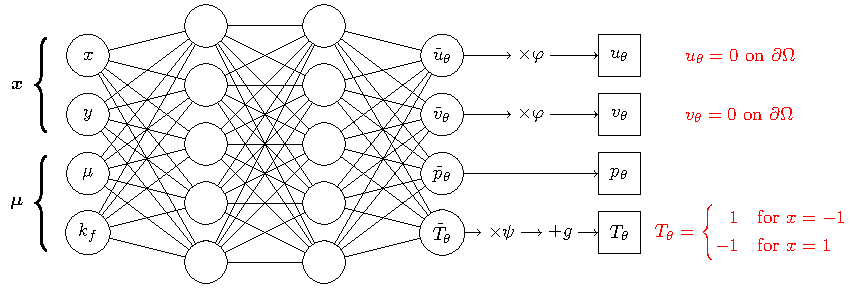
\includegraphics[width=0.85\linewidth]{images/pinn/network/network.pdf}
    \end{center}

    \vspace{-5pt}
    We consider two levelsets functions $\varphi_1$ and $\varphi_2$, and the linear function $g$ defined by
    \begin{equation*}
        \varphi_1(x,y) = (x-1)(x+1)(y-1)(y+1),
    \end{equation*}
    \begin{equation*}
        \varphi_2(x,y) = (x-1)(x+1) \quad \text{and} \quad g(x,y) = 1 - (x+1).
    \end{equation*}
\end{frame}

\begin{frame}{PINN training}
    \vspace{-4pt}
    \textbf{Approximate the solution of \eqref{eq:Pb} by a PINN :} Find the optimal weights $\theta^\star$, such that
	
    \vspace{-8pt}
    \begin{equation}
		\label{eq:opt_pb}
		\theta^\star = \argmin_{\theta}	\big( \; \textcolor{orange}{J_{inc}(\theta)} + \textcolor{orange}{J_{mom}(\theta)} + \textcolor{orange}{J_{ener}(\theta)} + \textcolor{darkred}{J_{ad}(\theta)} \; \big),
		\tag{$\mathcal{P}_\theta$}
	\end{equation}

    \vspace{-2pt}
	where the different cost functions\footnote[frame,1]{Discretized by a random process using Monte-Carlo method.} are defined by
	\vspace{5pt}

	\begin{minipage}{0.24\linewidth}
		\centering
		\textcolor{darkred}{adiabatic condition}
        
		\vspace{12pt}
		\textcolor{orange}{$3$ residual losses}
	\end{minipage}
	\begin{minipage}{0.68\linewidth}
		\centering
        \fcolorbox{darkred}{white}{
            $J_{ad}(\theta) =
            \int_{\mathcal{M}}\int_{\Gamma_\text{ad}} \big| \frac{\partial T_\theta(\bm{x},\bm{\mu})}{\partial n} \big|^2 d\bm{x} d\bm{\mu},$}
        
        \vspace{3pt}
		\fcolorbox{orange}{white}{
            $J_{\textbullet}(\theta) =
                \int_{\mathcal{M}}\int_{\Omega}
                \big| R_{\textbullet}(U_\theta(\bm{x},\bm{\mu});\bm{x},\bm{\mu}) \big|^2 d\bm{x} d\bm{\mu},$}
	\end{minipage}
    
    \vspace{5pt}
    with $U_\theta$ the parametric NN and $\textbullet$ the PDE considered (i.e. $inc$, $mom$ or $ener$).

    %\footnote[frame,2]{We consider a MLP with 5 hidden layers ($40,60,60,60,40$) and a 'sine' activation function. We train the PINN over $10000$ epochs ($3000$ ADAM / $7000$ LBFGS) with $40000$ collocation points in $\Omega$ and $30000$ points on the boundary $\partial\Omega\vert_{y=\pm 1}$.}
    
    \vspace{-7pt}
    \vspace{3pt}    
    \begin{center}
        \begin{minipage}{0.62\linewidth}
            \centering
            \vspace{-8pt}
            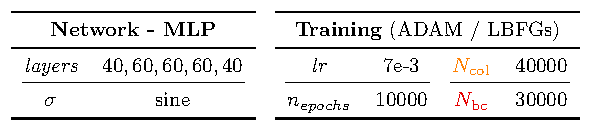
\includegraphics[width=0.94\linewidth]{images/pinn/training_param/training_param.pdf}
        \end{minipage}
        \begin{minipage}{0.36\linewidth}
            \centering
            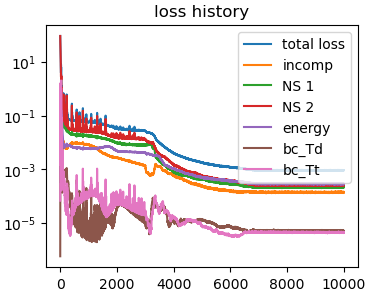
\includegraphics[width=0.84\linewidth]{images/pinn/training/test4_v5.png}
        \end{minipage}
    \end{center}
    
    \vspace{-8pt}
\end{frame}

\begin{frame}{Prediction on $\bm{\mu}^{(1)} = (0.1,0.1)$}
    \vspace{-4pt}
    \textbf{Prediction :} \begin{minipage}{0.26\linewidth}
        \centering
        $u_{1,\theta}$ \\
        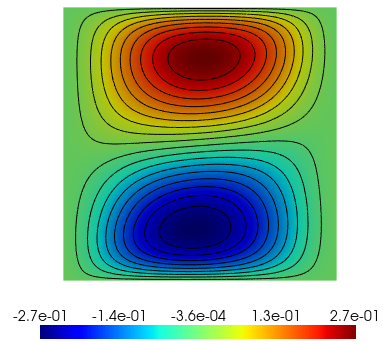
\includegraphics[width=0.95\linewidth]{images/pinn/training/PINN_plot_case4_v2_param1_u1.png}
    \end{minipage} \; \begin{minipage}{0.26\linewidth}
        \centering
        $u_{2,\theta}$ \\
        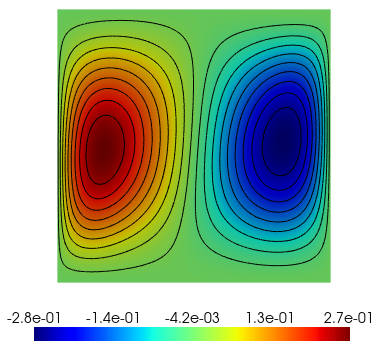
\includegraphics[width=0.95\linewidth]{images/pinn/training/PINN_plot_case4_v2_param1_u2.png}
    \end{minipage} \; \begin{minipage}{0.26\linewidth}
        \centering
        $T_\theta$ \\
        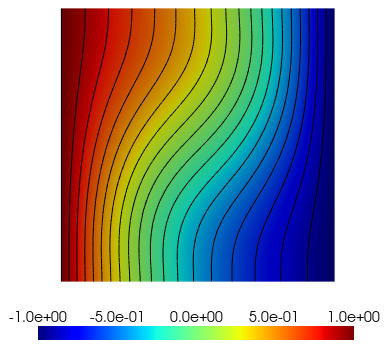
\includegraphics[width=0.95\linewidth]{images/pinn/training/PINN_plot_case4_v2_param1_T.png}
    \end{minipage}

    \vspace{8pt}

    \textbf{Error map :} \begin{minipage}{0.26\linewidth}
        \centering
        $u_{1,\text{ref}}-u_{1,\theta}$ \\
        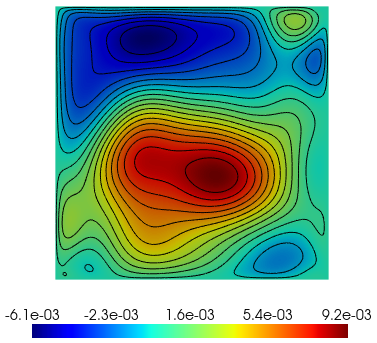
\includegraphics[width=0.95\linewidth]{images/pinn/training/PINN_error_plot_case4_v2_param1_u1.png}
    \end{minipage} \; \begin{minipage}{0.26\linewidth}
        \centering
        $u_{2,\text{ref}}-u_{2,\theta}$ \\
        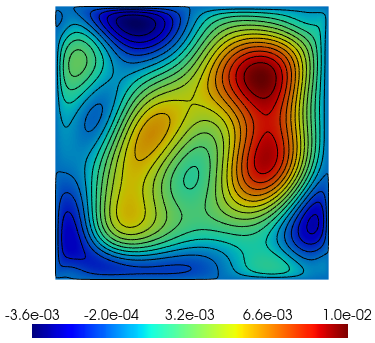
\includegraphics[width=0.95\linewidth]{images/pinn/training/PINN_error_plot_case4_v2_param1_u2.png}
    \end{minipage} \; \begin{minipage}{0.26\linewidth}
        \centering
        $T_\text{ref}-T_\theta$ \\
        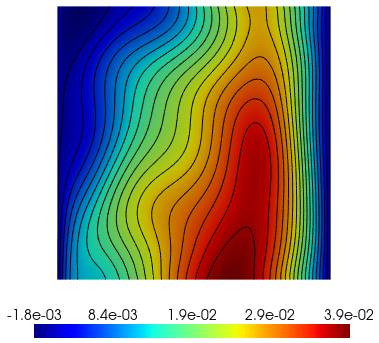
\includegraphics[width=0.95\linewidth]{images/pinn/training/PINN_error_plot_case4_v2_param1_T.png}
    \end{minipage}

    \vspace{8pt}

    \textbf{$L^2$ error :} \hspace{25pt} $2.98\times10^{-2} \hspace{42pt} 3.17\times10^{-2} \hspace{42pt}  3.90\times10^{-2}$

    \vspace{-2pt}
    \textbf{\small (relative)}
\end{frame}
	
	\section{Our hybrid method}
	\begin{frame}{$\phi$-FEM Method}
	\textbf{Main ideas :} \small
	
	\begin{minipage}[t]{0.48\linewidth}
		\begin{itemize}[\textbullet]
			\item Domain defined by a LevelSet Function $\phi$.
		\end{itemize}
		\centering
		\pgfimage[width=0.6\linewidth]{images/hybrid/PhiFEM_level_set.png}
	\end{minipage} \hfill
	\begin{minipage}[t]{0.48\linewidth}
		\begin{itemize}[\textbullet]
			\item We are looking for $w$ such that $u=\phi w+g$. \\
			Thus, the decoder is written as
			\begin{equation*}
				u_\theta(x)=\mathcal{D}_{\theta_w}(x) = \phi(x)\sum_{i=1}^{N}(\theta_w)_i\varphi_i+g(x)
			\end{equation*}
		\end{itemize}
	\end{minipage}

	\begin{itemize}[\textbullet]
		\item Mesh of a fictitious domain containing $\Omega$.
	\end{itemize}
	\begin{center}
		\begin{minipage}{0.43\linewidth}
			\centering
			\pgfimage[width=\linewidth]{images/more/PhiFEM_domain.png}
		\end{minipage} \hfill
		\begin{minipage}{0.1\linewidth}
			\centering
			\pgfimage[width=\linewidth]{images/more/PhiFEM_fleche.png} 
		\end{minipage} \hfill
		\begin{minipage}{0.43\linewidth}
			\centering
			\pgfimage[width=\linewidth]{images/more/PhiFEM_domain_considered.png}
		\end{minipage}
	\end{center}
\end{frame}

\begin{frame}{Impose exact BC in PINNs}
	\hl{A compléter !}
\end{frame}

\begin{frame}{Correct PINNs prediction with $\phi$FEM}
	\hl{A compléter !}
\end{frame}
	
	%	\section{Finite Element Methods}
	%	\subsection{Standard FEM method}

\begin{frame}{Presentation of standard FEM method}	    
    \textbf{Variational Problem :} $\quad\text{Find } u\in V \; | \; a(u,v)=l(v), \;\forall v\in V$
    
    with $V$ - Hilbert space, $a$ - bilinear form, $l$ - linear form.

    \vspace{10pt}

    \begin{minipage}[t]{0.76\linewidth}
        \textbf{Approach Problem :} $\quad \text{Find } u_h\in V_h \; | \; a(u_h,v_h)=l(v_h), \;\forall v_h\in V_h$
    
        with $\textbullet$ $u_h\in V_h$ an approximate solution of $u$, 
        
        $\textbullet V_h\subset V, \; dim V_h=N_h<\infty, \; (\forall h>0)$ 
        
       $\Rightarrow$ Construct a piecewise continuous functions space
       \vspace{-5pt}
       \begin{equation*}
           V_h:=P_{C,h}^k=\{v_h\in C^0(\bar{\Omega}), \forall K\in\mathcal{T}_h, {v_h}_{|K}\in\mathbb{P}_k\}
       \end{equation*}

       where $\mathbb{P}_k$ is the vector space of polynomials of total degree $\le k$.
    \end{minipage} \hfill \begin{minipage}[t][][b]{0.2\linewidth}
        \vspace{-5pt}
        \centering
        \pgfimage[width=0.9\linewidth]{images/fems/FEM_triangle_mesh.png}
        
        \footnotesize
        $\mathcal{T}_h = \left\{K_1,\dots,K_{N_e}\right\}$

        \tiny
        ($N_e$ : number of elements)
    \end{minipage}

    

    \vspace{10pt}

    Finding an approximation of the PDE solution $\Rightarrow$ solving the following linear system:
    \begin{equation*}
        AU=b
    \end{equation*}
    with
    \begin{equation*}
        A=(a(\varphi_i,\varphi_j))_{1\le i,j\le N_h}, \quad U=(u_i)_{1\le i\le N_h} \quad \text{and} \quad b=(l(\varphi_j))_{1\le j\le N_h}
    \end{equation*}
    where $(\varphi_1,\dots,\varphi_{N_h})$ is a basis of $V_h$.
\end{frame}
	
% \begin{frame}{Presentation of standard FEM method}	
%     \fcolorbox{white}{yellow}{Réduire à une seule diapo rapide !}
    
%     \textbf{Variational Problem :} 
%     \begin{equation*}
%         \text{Find } u\in V \text{ such that } a(u,v)=l(v), \;\forall v\in V
%     \end{equation*}
%     where $V$ is a Hilbert space, $a$ is a bilinear form and $l$ is a linear form.
    
%     \textbf{Approach Problem :} 
%     \begin{equation*}
%         \text{Find } u_h\in V_h \text{ such that } a(u_h,v_h)=l(v_h), \;\forall v_h\in V
%     \end{equation*}
%     with $u_h$ an approximate solution in $V_h$, a finite-dimensional space dependent on $h$ such that $\quad V_h\subset V, \; dimV_h = N_h<\infty, \; (\forall h>0)$ 
    
%     As $u_h=\sum_{i=1}^{N_h}u_i\varphi_i$ with $(\varphi_1,\dots,\varphi_{N_h})$ a basis of $V_h$, finding an approximation of the PDE solution implies solving the following linear system:
%     \begin{equation*}
%         AU=b
%     \end{equation*}
%     with
%     \begin{equation*}
%         A=(a(\varphi_i,\varphi_j))_{1\le i,j\le N_h}, \quad U=(u_i)_{1\le i\le N_h} \quad \text{and} \quad b=(l(\varphi_j))_{1\le j\le N_h}
%     \end{equation*}
% \end{frame}

% \begin{frame}{In practice}
%     \begin{enumerate}[\ding{217}]
%         \item \begin{minipage}[t]{0.68\linewidth}
%             Construct a mesh of our $\Omega$ geometry with a family of elements (in 2D: triangle, rectangle; in 3D: tetrahedron, parallelepiped, prism) defined by
%             $$\mathcal{T}_h = \left\{K_1,\dots,K_{N_e}\right\}$$
%             where $N_e$ is the number of elements. \\
%         \end{minipage} \begin{minipage}[t][][b]{0.28\linewidth}
%             \centering
%             \qquad \pgfimage[width=0.8\linewidth]{images/fems/FEM_triangle_mesh.png}
%         \end{minipage}
%         (Importance of geometric quality)
%         \item Construct a space of piece-wise affine continuous functions, defined by
%         \begin{equation*}
%             V_h:=P_{C,h}^k=\{v_h\in C^0(\bar{\Omega}), \forall K\in\mathcal{T}_h, {v_h}_{|K}\in\mathbb{P}_k\}
%         \end{equation*}
%         where $\mathbb{P}_k$ is the vector space of polynomials of total degree less than or equal to $k$.
%     \end{enumerate}
    
% \end{frame}

\subsection{$\phi$-FEM method}

\begin{frame}{Problem}
    Let $u=\phi w+g$ such that
    $$\left\{\begin{aligned}
        -\Delta u &= f, \; \text{in } \Omega, \\
        u&=g, \; \text{on } \Gamma, \\
    \end{aligned}\right.$$
    where $\phi$ is the level-set function and $\Omega$ and $\Gamma$ are given by :
    \begin{center}
        \pgfimage[width=0.5\linewidth]{images/fems/PhiFEM_level_set.png}
    \end{center}
    The level-set function $\phi$ is supposed to be known on $\mathbb{R}^d$ and sufficiently smooth. \\
    For instance, the signed distance to $\Gamma$ is a good candidate.

    \vspace{5pt}

    \footnotesize
    \textit{Remark :} Thanks to $\phi$ and $g$, the conditions on the boundary are respected.
\end{frame}

\begin{frame}{Fictitious domain}
    \setstretch{0.5}

    \vspace{10pt}
    
    \begin{center}
        \begin{minipage}{0.43\linewidth}
            \centering
            \pgfimage[width=\linewidth]{images/fems/PhiFEM_domain.png}
        \end{minipage} \hfill
        \begin{minipage}{0.1\linewidth}
            \centering
            \pgfimage[width=\linewidth]{images/fems/PhiFEM_fleche.png} 
        \end{minipage} \hfill
        \begin{minipage}{0.43\linewidth}
            \centering
            \pgfimage[width=\linewidth]{images/fems/PhiFEM_domain_considered.png}
        \end{minipage}
    \end{center}

    \begin{enumerate}[\ding{217}]
        \item $\phi_h$ : approximation of $\phi$ \\ 
        \item $\Gamma_h=\{\phi_h=0\}$ : approximate boundary of $\Gamma$
        \item $\Omega_h$ : computational mesh
        \item $\partial\Omega_h$ : boundary of $\Omega_h$ ($\partial\Omega_h \ne \Gamma_h$)
    \end{enumerate}	
    
    % \begin{minipage}{0.6\linewidth}
    %     \begin{enumerate}[\ding{217}]
    %         \item $\mathcal{O}$ : fictitious domain such that $\Omega\subset\mathcal{O}$
    %         \item $\mathcal{T}_h^\mathcal{O}$ : simple quasi-uniform mesh on $\mathcal{O}$
    %         \item $\phi_h=I_{h,\mathcal{O}}^{(l)}(\phi)\in V_{h,\mathcal{O}}^{(l)}$ : approximation of $\phi$ \\ 
    %         with $I_{h,\mathcal{O}}^{(l)}$ the standard Lagrange interpolation operator on
    %         $$V_{h,\mathcal{O}}^{(l)}=\left\{v_h\in H^1(\mathcal{O}):v_{h|_T}\in\mathbb{P}_l(T) \;  \forall T\in\mathcal{T}_h^\mathcal{O}\right\}$$
    %         \item $\Gamma_h=\{\phi_h=0\}$ : approximate boundary of $\Gamma$
    %         \item $\mathcal{T}_h$ : sub-mesh of $\mathcal{T}_h^\mathcal{O}$ defined by
    %         $$\mathcal{T}_h=\left\{T\in \mathcal{T}_h^\mathcal{O}:T\cap\{\phi_h<0\}\ne\emptyset\right\}$$
    %         \item $\Omega_h$ : domain covered by the $\mathcal{T}_h$ mesh defined by
    %         $$\Omega_h=\left(\cup_{T\in\mathcal{T}_h}T\right)^O$$
    %         ($\partial\Omega_h$ its boundary)
    %     \end{enumerate}			
    % \end{minipage}
    
    \footnotesize
    \; \\
    \textit{Remark :} $n_{vert}$ will denote the number of vertices in each direction for $\mathcal{O}$
\end{frame}

\begin{frame}{Facets and Cells sets}

    \vspace{15pt}

    \begin{center}
        \begin{minipage}{0.48\linewidth}
            \centering
            \pgfimage[width=\linewidth]{images/fems/PhiFEM_boundary_cells.png}
        \end{minipage} \hfill
        \begin{minipage}{0.48\linewidth}
            \centering
            \pgfimage[width=\linewidth]{images/fems/PhiFEM_boundary_edges.png}
        \end{minipage}
    \end{center}

    \begin{enumerate}[\ding{217}]
        \item $\mathcal{T}_h^\Gamma$ : mesh elements cut by $\Gamma_h$
        \item $\mathcal{F}_h^\Gamma$ : collects the interior facets of $\mathcal{T}_h^\Gamma$ \\
        (either cut by $\Gamma_h$ or belonging to a cut mesh element)
    \end{enumerate}

    % \begin{minipage}{0.6\linewidth}
    %     \begin{enumerate}[\ding{217}]
    %         \item $\mathcal{T}_h^\Gamma\subset \mathcal{T}_h$ : contains the mesh elements cut by $\Gamma_h$, i.e. 
    %         \begin{equation*}
    %             \mathcal{T}_h^\Gamma=\left\{T\in\mathcal{T}_h:T\cap\Gamma_h\ne\emptyset\right\},
    %         \end{equation*}
    %         \item $\Omega_h^\Gamma$ : domain covered by the $\mathcal{T}_h^\Gamma$ mesh, i.e.
    %         \begin{equation*}
    %             \Omega_h^\Gamma=\left(\cup_{T\in\mathcal{T}_h^\Gamma}T\right)^O
    %         \end{equation*}
    %         \item $\mathcal{F}_h^\Gamma$ : collects the interior facets of $\mathcal{T}_h$ either cut by $\Gamma_h$ or belonging to a cut mesh element, i.e.
    %         \begin{align*}
    %             \mathcal{F}_h^\Gamma=\left\{E\;(\text{an internal facet of } \mathcal{T}_h) \text{ such that }\right. \\
    %             \left. \exists T\in \mathcal{T}_h:T\cap\Gamma_h\ne\emptyset \text{ and } E\in\partial T\right\}
    %         \end{align*}
    %     \end{enumerate}
    % \end{minipage}
\end{frame}

\begin{frame}{$\phi$-FEM Method - Poisson problem}
    \textbf{Approach Problem :} Find $w_h\in V_h^{(k)}$ such that 
    $$a_h(w_h,v_h) = l_h(v_h) \quad \forall v_h \in V_h^{(k)}$$
    where
    $$a_h(w,v)=\int_{\Omega_h} \nabla (\phi_h w) \cdot \nabla (\phi_h v) - \int_{\partial\Omega_h} \frac{\partial}{\partial n}(\phi_h w)\phi_h v+G_h(w,v),$$
    $$l_h(v)=\int_{\Omega_h} f \phi_h v + G_h^{rhs}(v) \qquad \qquad \color{white}\text{Stabilization terms}$$
    and 
    $$V_h^{(k)}=\left\{v_h\in H^1(\Omega_h):v_{h|_T}\in\mathbb{P}_k(T), \; \forall T\in\mathcal{T}_h\right\}.$$
    For the non homogeneous case, we replace
    $$u=\phi w \quad \rightarrow \quad u=\phi w+g$$ 
    by supposing that $g$ is currently given over the entire $\Omega_h$.
\end{frame}

\begin{frame}[noframenumbering]{$\phi$-FEM Method - Poisson problem}
    \textbf{Approach Problem :} Find $w_h\in V_h^{(k)}$ such that 
    $$a_h(w_h,v_h) = l_h(v_h) \quad \forall v_h \in V_h^{(k)}$$
    where
    $$a_h(w,v)=\int_{\Omega_h} \nabla (\phi_h w) \cdot \nabla (\phi_h v) - \int_{\partial\Omega_h} \frac{\partial}{\partial n}(\phi_h w)\phi_h v+\fcolorbox{blue}{white}{$G_h(w,v)$},$$
    $$l_h(v)=\int_{\Omega_h} f \phi_h v + \fcolorbox{blue}{white}{$G_h^{rhs}(v)$} \qquad \qquad \color{blue}\text{Stabilization terms}$$
    and 
    $$V_h^{(k)}=\left\{v_h\in H^1(\Omega_h):v_{h|_T}\in\mathbb{P}_k(T), \; \forall T\in\mathcal{T}_h\right\}.$$
    For the non homogeneous case, we replace
    $$u=\phi w \quad \rightarrow \quad u=\phi w+g$$ 
    by supposing that $g$ is currently given over the entire $\Omega_h$.
\end{frame}

\begin{frame}{Stabilization terms}
    \begin{center}
        \centering
        \pgfimage[width=\linewidth]{images/fems/PhiFEM_stab_terms.png}
    \end{center}
    \small
    \underline{1st term :} ensure continuity of the solution by penalizing gradient jumps. \\
    $\rightarrow$ Ghost penalty [Burman, 2010] \\
    \underline{2nd term :} require the solution to verify the strong form on $\Omega_h^\Gamma$. \\
    \normalsize
    \textbf{Purpose :} 
    \begin{enumerate}[\ding{217}]
        \item reduce the errors created by the "fictitious" boundary 
        \item ensure the correct condition number of the finite element matrix
        \item restore the coercivity of the bilinear scheme
    \end{enumerate}
\end{frame}
        

	
%	\section{Internship results}
%	\subsection{Correction Methods}

% \begin{frame}{Correction Methods}
%     We are given $u_\theta$ the FNO prediction (for the problem under consideration).
    
%     \begin{minipage}{0.48\linewidth}
%         \textbf{By adding :}
    
%         We will consider
%         \begin{equation*}
%             \tilde{u}=u_\theta+\tilde{C}
%         \end{equation*}

%         We want $\tilde{C}: \Omega \rightarrow \mathbb{R}^d$ such that
%         \begin{equation}
%             \left\{\begin{aligned}
%                 -\Delta \tilde{C}&=\tilde{f}, \; &&\text{on } \Omega, \\
%                 \tilde{C}&=0, \; &&\text{in } \Gamma.
%             \end{aligned}\right. \tag{$\mathcal{C}_{+}$} %\label{corr_add}
%         \end{equation}
%         with $\tilde{f}=f+\Delta u_\theta$ and $\tilde{C}=\phi C$ for the $\phi$-FEM method.
        
%         \small
%         \textit{Remark :} In practice, it may be useful to integrate by parts the term containing $\Delta u_\theta$.
%     \end{minipage} \quad
%     \begin{minipage}{0.48\linewidth}
%         \textbf{By multiplying :}
        
%         \small
%         \textcolor{white}{Find $\hat{u} : \Omega \rightarrow \mathbb{R}^d$ such that
% 		\begin{equation}
% 			\left\{
% 			\begin{aligned}
% 				-\Delta \hat{u} = f, \; &&\text{in } \; \Omega, \\
% 				\hat{u}=g+m, \; &&\text{on } \; \Gamma,
% 			\end{aligned}
% 			\right. \tag{$\mathcal{P}^\mathcal{M}$} \label{pb_reh}
% 		\end{equation}
% 		with $\hat{u}=u+m$ ($m$ a constant).}

%         \normalsize
%         We will consider
%         \begin{equation*}
%             \tilde{u}=u_\theta C
%         \end{equation*}
%         \textcolor{white}{with $\hat{u_\theta}=u_\theta+m$.}
        
%         We want $C: \Omega \rightarrow \mathbb{R}^d$ such that
%         \begin{equation*}
%             \left\{\begin{aligned}
%                 &-\Delta (u_\theta C)=f, \; &&\text{on } \Omega, \\
%                 &C=1, \; &&\text{on } \; \Gamma.
%             \end{aligned}\right. \tag{$\mathcal{C}_\times$} %\label{corr_mult}
%         \end{equation*}
%     \end{minipage}
% \end{frame}

\begin{frame}{Correction Methods}
    We are given $u_\theta$ the FNO prediction (for the problem under consideration).
    
    \begin{minipage}{0.48\linewidth}
        \textbf{By adding :}
    
        We will consider
        \begin{equation*}
            \tilde{u}=u_\theta+\fcolorbox{blue}{white}{$\tilde{C}$}\textcolor{blue}{\approx 0}
        \end{equation*}

        We want $\tilde{C}: \Omega \rightarrow \mathbb{R}^d$ such that
        \begin{equation}
            \left\{\begin{aligned}
                -\Delta \tilde{C}&=\tilde{f}, \; &&\text{in } \Omega, \\
                \tilde{C}&=0, \; &&\text{on } \Gamma.
            \end{aligned}\right. \tag{$\mathcal{C}_{+}$} %\label{corr_add}
        \end{equation}
        with $\tilde{f}=f+\Delta u_\theta$ and $\tilde{C}=\phi C$ for the $\phi$-FEM method.
        
        \small
        \textit{Remark :} In practice, it may be useful to integrate by parts the term containing $\Delta u_\theta$.
    \end{minipage} \quad
    \begin{minipage}{0.48\linewidth}
        \textbf{By multiplying :}
        
        \small
        \textcolor{white}{Find $\hat{u} : \Omega \rightarrow \mathbb{R}^d$ such that
		\begin{equation}
			\left\{
			\begin{aligned}
				-\Delta \hat{u} = f, \; &&\text{in } \; \Omega, \\
				\hat{u}=g+m, \; &&\text{on } \; \Gamma,
			\end{aligned}
			\right. \tag{$\mathcal{P}^\mathcal{M}$} %\label{pb_reh}
		\end{equation}
		with $\hat{u}=u+m$ ($m$ a constant).}

        \normalsize
        We will consider
        \begin{equation*}
            \tilde{u}=u_\theta \fcolorbox{blue}{white}{$C$}\textcolor{blue}{\approx 1}
        \end{equation*}
        \textcolor{white}{with $\hat{u_\theta}=u_\theta+m$.}
        
        We want $C: \Omega \rightarrow \mathbb{R}^d$ such that
        \begin{equation*}
            \left\{\begin{aligned}
                &-\Delta (u_\theta C)=f, \; &&\text{on } \Omega, \\
                &C=1, \; &&\text{on } \; \Gamma.
            \end{aligned}\right. \tag{$\mathcal{C}_\times$} \label{corr_mult}
        \end{equation*}
    \end{minipage}
\end{frame}

\begin{frame}[noframenumbering]{Correction Methods}
    We are given $u_\theta$ the FNO prediction (for the problem under consideration).
    
    \begin{minipage}{0.48\linewidth}
        \textbf{By adding :}
    
        We will consider
        \begin{equation*}
            \tilde{u}=u_\theta+\tilde{C}
        \end{equation*}

        We want $\tilde{C}: \Omega \rightarrow \mathbb{R}^d$ such that
        \begin{equation}
            \left\{\begin{aligned}
                -\Delta \tilde{C}&=\tilde{f}, \; &&\text{in } \Omega, \\
                \tilde{C}&=0, \; &&\text{on } \Gamma.
            \end{aligned}\right. \tag{$\mathcal{C}_{+}$} \label{corr_add}
        \end{equation}
        with $\tilde{f}=f+\Delta u_\theta$ and $\tilde{C}=\phi C$ for the $\phi$-FEM method.
        
        \small
        \textit{Remark :} In practice, it may be useful to integrate by parts the term containing $\Delta u_\theta$.
    \end{minipage} \quad
    \begin{minipage}{0.48\linewidth}
        \textbf{By multiplying \textcolor{red}{- elevated problem} :}
        
        \small
        \textcolor{red}{Find $\hat{u} : \Omega \rightarrow \mathbb{R}^d$ such that
		\begin{equation}
			\left\{
			\begin{aligned}
				-\Delta \hat{u} = f, \; &&\text{in } \; \Omega, \\
				\hat{u}=g+m, \; &&\text{on } \; \Gamma,
			\end{aligned}
			\right. \tag{$\mathcal{P}^{\mathcolor{red}{\mathcal{M}}}$} \label{pb_reh}
		\end{equation}
		with $\hat{u}=u+m$ ($m$ a constant).}

        \normalsize
        We will consider
        \begin{equation*}
            \tilde{u}=\uchapeau{u_\theta} C
        \end{equation*}
        \textcolor{red}{with $\hat{u_\theta}=u_\theta+m$.}
        
        We want $C: \Omega \rightarrow \mathbb{R}^d$ such that
        \begin{equation*}
            \left\{\begin{aligned}
                &-\Delta (\uchapeau{u_\theta} C)=f, \; &&\text{in } \Omega, \\
                &C=1, \; &&\text{on } \; \Gamma.
            \end{aligned}\right. \tag{$\mathcal{C}_\times^{\mathcolor{red}{\mathcal{M}}}$} \label{corr_mult_reh}
        \end{equation*}
    \end{minipage}
\end{frame}

\subsection{Results - with FNO}

\begin{frame}{Explanation}
    \vspace{5pt}
    \begin{minipage}{0.48\linewidth}
        \textbf{Train a FNO :}
        
        \pgfimage[width=\linewidth]{images/internship/FNO/Training.png}
    \end{minipage} \quad
    \begin{minipage}{0.48\linewidth}
        \textbf{Correct the predictions of the FNO :}
        
        \pgfimage[width=\linewidth]{images/internship/FNO/Correction.png}
    \end{minipage}

    \vspace{15pt}
    \textbf{Some important points on the FNO :}
    \begin{enumerate}[\ding{217}]        
        \item widely used in PDE solving and constitute an active field of research
        \item FNO are Neural Operator networks : Unlike standard neural networks, which learn using inputs and outputs of fixed dimensions, neural operators \textbf{learn operators, which are mappings between spaces of functions}.
        \item \textbf{Mesh resolution independent :} can be evaluated at almost any data resolution without the need for retraining
    \end{enumerate}
\end{frame}

\begin{frame}{Correction on a FNO prediction - $\phi$-FEM}
    We consider an unknown solution on the circle with $f$ Gaussian \eqref{sol1}, $n_{vert}=63$, $n_{data}=1000$ (including validation sample) and $n_{test}=100$. 

    \vspace{10pt}
    \begin{minipage}{0.38\linewidth}
        Training on 4000 epochs (bs=64,lr=0.01) :
        \centering
        \pgfimage[width=0.9\linewidth]{images/internship/FNO/misfits_f_gaussienne.png}
    \end{minipage}
    \begin{minipage}{0.58\linewidth}
        Correction with the different methods :
        \centering
        \pgfimage[width=\linewidth]{images/internship/FNO/corr_boxplot.png}
    \end{minipage}	
    
    \vspace{5pt}
    \footnotesize
    \textbf{Remark :} We should try to reduce the resolution for correction, maybe we will gain in the time-to-error ratio.
\end{frame}

\subsection{Other results}

% \begin{frame}{Precision of the prediction - FEM}    
%     We consider the trigonometric solution on the circle \eqref{sol2} with

%     \begin{minipage}{0.4\linewidth}
%         $\; \textbullet$ $u_{ex}$ : the exact solution of \eqref{pb_initial}
        
%         \textcolor{white}{$\; \textbullet$ $u_\theta$ : a disturbed solution of }
        
%         $(S,f,\varphi)=(0.5,1,0)$
        
%         \textcolor{white}{$(S_p,f_p,\varphi_p)=(0.5,2,0)$}
        
%         \textbf{Exact solution :} $u_\theta=u_{ex}\in\mathbb{P}^{10}$

%         Correction with FEM ($n_{vert}=32$) :
        
%         \pgfimage[width=\linewidth]{images/internship/precision/exact_sol/exact_fem_circle_nvert32_fleche}
%     \end{minipage}
    
% \end{frame}

% \begin{frame}[noframenumbering]{Precision of the prediction - FEM}    
%     We consider the trigonometric solution on the circle \eqref{sol2} with

%     \begin{minipage}{0.4\linewidth}
%         $\; \textbullet$ $u_{ex}$ : the exact solution of \eqref{pb_initial}
        
%         \textcolor{white}{$\; \textbullet$ $u_\theta$ : a disturbed solution of }
        
%         $(S,f,\varphi)=(0.5,1,0)$
        
%         \textcolor{white}{$(S_p,f_p,\varphi_p)=(0.5,2,0)$}
        
%         \textbf{Exact solution :} $u_\theta=u_{ex}\in\mathbb{P}^{10}$

%         Correction with FEM ($n_{vert}=32$) :
        
%         \pgfimage[width=\linewidth]{images/internship/precision/exact_sol/exact_fem_circle_nvert32_fleche}

%         \textcolor{red}{Correction with FEM ($n_{vert}=100$) :}
        
%         \pgfimage[width=\linewidth]{images/internship/precision/exact_sol/exact_fem_circle_nvert100_colorbox}
%     \end{minipage}	
% \end{frame}

% \begin{frame}[noframenumbering]{Precision of the prediction - FEM}    
%     We consider the trigonometric solution on the circle \eqref{sol2} with

%     \begin{minipage}{0.4\linewidth}
%         $\; \textbullet$ $u_{ex}$ : the exact solution of \eqref{pb_initial}
        
%         \textcolor{red}{$\; \textbullet$ $u_\theta$ : a disturbed solution}
        
%         $(S,f,\varphi)=(0.5,1,0)$
        
%         \textcolor{red}{$(S_p,f_p,\varphi_p)=(0.5,2,0)$}
        
%         \textbf{Exact solution :} $u_\theta=u_{ex}\in\mathbb{P}^{10}$
        
%         Correction with FEM ($n_{vert}=32$) :

%         \centering
%         \pgfimage[width=0.9\linewidth]{images/internship/precision/exact_sol/exact_fem_circle_nvert32}

%         \raggedright
%         Correction with FEM ($n_{vert}=100$) :

%         \centering
%         \pgfimage[width=0.9\linewidth]{images/internship/precision/exact_sol/exact_fem_circle_nvert100}
%     \end{minipage} \quad
%     \fcolorbox{red}{white}{\begin{minipage}{0.54\linewidth}
%         \textbf{Disturbed solution :} $u_\theta=u_{ex}+\epsilon P\in\mathbb{P}^{k}$
        
%         with $\epsilon$ a real number and $P$ the perturbation.
        
%         Correction by adding with FEM ($n_{vert}=32$) :

%         \centering
%         \pgfimage[width=0.8\linewidth]{images/internship/precision/disturbed_sol/disturbed_fem_circle_nvert32_add}

%         \raggedright
%         Results for $k=10$ :
        
%         \pgfimage[width=\linewidth]{images/internship/precision/disturbed_sol/norms_P10_line}

%         with $\tilde{u}$ the solution obtained with the correction by addition, apply on $u_\theta$. 
%     \end{minipage}}

%     \footnotesize
%     \textit{Remark :} In practice, the expression of $u_{ex}$ will be chosen as the expression of $P$ (with the perturbation parameters $(S_p,f_p,\varphi_p)$). Consider $\varphi_p=0$ so that $P=0$ on $\Gamma$ and therefore $\tilde{\phi}=0$ on $\Gamma$.
% \end{frame}

\begin{frame}{Precision of the prediction - FEM}    
    We consider the trigonometric solution on the circle \eqref{sol2} with
    $$u_{ex}(x,y)=S\sin\left(8\pi f\left((x-0.5)^2+(y-0.5)^2\right)+\varphi\right)$$
    with $S=0.5$ and $\varphi=0$.

    \textbf{Exact solution :} Testing different correction methods for different frequencies.

    $$u_\theta=u_{ex}\in\mathbb{P}^{10} \; \rightarrow \; \tilde{u}\in\mathbb{P}^1$$

    \begin{center}     
        Correction with FEM ($n_{vert}=100$) :
        
        \pgfimage[width=0.6\linewidth]{images/internship/precision/exact_sol/exact_fem_circle_nvert100_colorbox}
    \end{center}
\end{frame}

\begin{frame}{Precision of the prediction - FEM}  
    We consider $(S,f,\varphi)=(0.5,1,0)$.

    \textbf{Disturbed solution :} Testing different $\epsilon$ and different degree $k$.
    $$u_\theta=u_{ex}+\epsilon P\in\mathbb{P}^{k} \; \rightarrow \; \tilde{u}\in\mathbb{P}^1$$
    with $\epsilon$ a real number and $P$ a perturbation.
    
    \begin{minipage}{0.58\linewidth}        
        Correction \eqref{corr_add} with FEM ($n_{vert}=32$) :

        \centering
        \pgfimage[width=\linewidth]{images/internship/precision/disturbed_sol/disturbed_fem_circle_nvert32_add}
    \end{minipage} \hfill
    \begin{minipage}{0.38\linewidth}        
        \vspace{-5pt}
        Results for $k=10$ :

        \centering
        \pgfimage[width=0.5\linewidth]{images/internship/precision/disturbed_sol/norms_P10}
    \end{minipage}

    \footnotesize
    \textit{Remark :} $P(x,y)=S_p\sin\left(8\pi f_p\left((x-0.5)^2+(y-0.5)^2\right)+\varphi_p\right)$ with $(S_p,f_p,\varphi_p)=(0.5,2,0)$
\end{frame}

\begin{frame}{Theoretical results - FEM}
    \textbf{Correction by multiplication on the elevated problem :} We consider 
        
    \begin{itemize}
        \item \textcolor{red}{$\hat{u_{ex}}=u_{ex}+m$} : the exact solution of \eqref{pb_reh}
        \item \textcolor{red}{$\hat{u_\theta} = u_\theta+m$} : a disturbed solution of \eqref{pb_reh}.
        \item $\tilde{u_h}=\hat{u_\theta}C_h$ : the approximate solution of \eqref{corr_mult_reh}
    \end{itemize}

    % We show that $\qquad \left|\left|\hat{u_{ex}}-\tilde{u_h}\right|\right|_0\le ch^{k+1}||\hat{u_\theta}||_\infty\left|C\right|_{k+1}$
        
    \begin{minipage}{0.48\linewidth}
        \setstretch{0.5}
        \textbf{1.} When m tends to infinity : 
            \begin{center}
                solution of \eqref{corr_mult_reh} $\rightarrow$ solution of \eqref{corr_add}
            \end{center}

            \small
            \textbf{Results :} $n_{vert}=32$, $\epsilon=0.001$ \\
            
            \centering
            \pgfimage[width=0.6\linewidth]{images/internship/theo_results/first/fig_fem_circle.png}
    \end{minipage} \;
    \begin{minipage}{0.48\linewidth}
        \setstretch{0.5}
        \textbf{2.} For $m$ sufficiently large : $C_{ex}=\hat{u_{ex}}/\hat{u_\theta}$
            \begin{equation*}
                \left|\left|C_{ex}-C_h\right|\right|_{0,\Omega}\le ch^{k+1}\epsilon\left|\left|P''\right|\right|_{0,\Omega}
            \end{equation*}

            \small
            \textbf{Results :} $n_{vert}=32$, $\epsilon=0.001$, $f_p=2$ \\
    
            \centering
            \pgfimage[width=0.6\linewidth]{images/internship/theo_results/second/fig_fem_circle.png}
    \end{minipage}
    
    
\end{frame}
%	
%	\section{PhD results}
%	\begin{frame}{Explanation}
    \textbf{Context :} Need $u_\theta\in\mathbb{P}^k$ with $k$ of high degree

    \begin{center}
        \begin{minipage}{0.28\linewidth}
            \centering
            FNO \\
            (on a regular grid) 
        \end{minipage} $\rightarrow$ \begin{minipage}{0.35\linewidth}
            \centering
            NN which can predict \\
            solution at any point
        \end{minipage}
    \end{center}

    \textbf{Solutions :}

    \vspace{2pt}
    
    \begin{minipage}{0.48\linewidth}
        \; \\
        \textbf{1. MLP} - Multi-Layer Perceptron \\
        (= Fully connected)

        \centering
        \pgfimage[width=0.9\linewidth]{images/phd/MLP_schema.png}

        \raggedright
        \textit{Problem :} As the prediction is injected into an FEM solver, the accuracy of the derivatives is very important.
    \end{minipage} \quad
    \begin{minipage}{0.48\linewidth}
        \textbf{2. PINNs} - MLP with a physical loss
        \begin{center}
            $loss = mse(\Delta (\phi(x_i,y_i)w_{\theta,i})+f_i)$

            \vspace{1.5pt}
        
            \pgfimage[width=0.5\linewidth]{images/phd/PINNs_explanation.png}
        \end{center}

        with $(x_i,y_i)\in\mathcal{O}$.

        \textit{Remark :} We impose exact boundary conditions. \\
    \end{minipage}
\end{frame}

\begin{frame}{PINNs Training}
    We consider the solution on the circle defined in \eqref{sol3} and defined by
    \begin{equation*}
        u_{ex}(x,y)=\phi(x,y)\sin(x)\exp(y)
    \end{equation*}
    We train a PINNs with 4 layers of 20 neurons over 10000 epochs (with $n_{pts}=2000$ points selected uniformly over $\mathcal{O}$).

    \centering
    \pgfimage[width=0.9\linewidth]{images/phd/solution_config0.png}

    {\fontencoding{U}\fontfamily{futs}\selectfont\char 49\relax} We consider a single problem ($f$ fixed) on a single geometry ($\phi$ fixed).

    \raggedright    
    $||u_{ex}-u_\theta||_{0,\Omega}^{(rel)}\approx 2.81e-3$
\end{frame}

\begin{frame}{Derivatives}
    \; \\
    
    \centering
    \pgfimage[width=0.75\linewidth]{images/phd/derivatives_x.png}
\end{frame}

\begin{frame}{Correction by addition}
    $u_\theta\in\mathbb{P}^{10} \; \rightarrow \; \tilde{u}\in\mathbb{P}^1$

    \begin{minipage}{0.5\linewidth}
        \centering
        \pgfimage[width=\linewidth]{images/phd/time_precision.png}
    
        \raggedright
        FEM / $\phi$-FEM : $n_{vert}\in\{8,16,32,64,128\}$
        
        Corr : $n_{vert}\in\{5,10,15,20,25,30\}$
    \end{minipage} \quad
    \begin{minipage}{0.46\linewidth}
        \centering
        \pgfimage[width=\linewidth]{images/phd/results_time_1e-4.png}

        \small\raggedright
        $\textbullet$ \textbf{mesh} - FEM : construct the mesh \\
        ($\phi$-FEM : construct cell/facet sets) \\
        $\textbullet$ \textbf{u\_PINNs} - get $u_\theta$ in $\mathbb{P}^{10}$ freedom degrees \\
        $\textbullet$ \textbf{assemble} - assemble the FE matrix \\
        $\textbullet$ \textbf{solve} - resolve the linear system
    \end{minipage}

    \small
    \textit{Remark :} The stabilisation parameter $\sigma$ of the $\phi$-FEM method has a major impact on the error obtained.
\end{frame}
	
	\section{Conclusion} %perspectives
	
	\begin{frame}[label={lastslide}]{Conclusion}
		\hl{A compléter !}
	\end{frame}
	
	\section{Bibliography}
	
	{\setbeamertemplate{footline}{} 
		\begin{frame}{Bibliography}
			\small
			% \vspace{30pt}
			% \setstretch{0.2}
			% \AtNextBibliography{\small}
			\printbibliography[heading=none]
		\end{frame}
	}
	\addtocounter{framenumber}{-2} 
	
	\appendix
	
	\begin{frame}{\appendixname~\insertframenumber~: Encoding - FEMs}\phantomsection\label{frame:encoding_fems}
	
	Pourquoi ?
\end{frame}

%\begin{frame}{Architecture of the FNO}
%    \begin{center}
%        \centering
%        \pgfimage[width=\linewidth]{images/more/FNO/FNO_schema.png}
%    \end{center}
%    \textbf{Input $X$} of shape (bs,ni,nj,nk) \qquad \qquad \textbf{Output $Y$} of shape (bs,ni,nj,1) \\
%    with bs the batch size, ni and nj the grid resolution and nk the number of channels.
%\end{frame}
%
%\begin{frame}{Description of the FNO architecture}
%    \begin{center}
%        \centering
%        \pgfimage[width=\linewidth]{images/more/FNO/FNO_schema_moitie1.png}
%    \end{center}
%    \begin{enumerate}[\ding{217}]
%        \item perform a $P$ transformation, to move to a space with more channels (to build a sufficiently rich representation of the data)
%        \item apply $L$ Fourier layers defined by
%        $$\mathcal{H}_\theta^l(\tilde{X})=\sigma\left(\mathcal{C}_\theta^l(\tilde{X})+\mathcal{B}_\theta^l(\tilde{X})\right),\; l=1,\dots,L$$
%        with $\tilde{X}$ the input of the current layer and
%        \begin{itemize}
%            \item $\sigma$ an activation function (ReLU or GELU)
%            \item $\mathcal{C}_\theta^l$ : convolution sublayer (convolution performed by Fast Fourier Transform)
%            \item $\mathcal{B}_\theta^l$ : "bias-sublayer"
%        \end{itemize}
%        \item return to the target dimension by performing a $Q$ transformation (in our case, the number of output channels is 1)
%    \end{enumerate}
%\end{frame}
%
%\begin{frame}{Fourier Layer Structure}
%    \setstretch{0.5}
%    \textbf{Convolution sublayer : } \quad $\mathcal{C}_\theta^l(X)=\mathcal{F}^{-1}(\mathcal{F}(X)\cdot\hat{W})$ \quad
%    \begin{minipage}{0.3\linewidth}
%        \vspace{-15pt}
%        \centering
%        \pgfimage[width=\linewidth]{images/more/FNO/FNO_schema_moitie2.png}
%    \end{minipage}
%    \begin{enumerate}[\ding{217}]
%        \item $\hat{W}$ : a trainable kernel
%        \item $\mathcal{F}$ : 2D Discrete Fourier Transform (DFT) defined by
%        \begin{equation*}
%            \mathcal{F}(X)_{ijk}=\frac{1}{ni}\frac{1}{nj}\sum_{i'=0}^{ni-1}\sum_{j'=0}^{nj-1}X_{i'j'k}e^{-2\sqrt{-1}\pi\left(\frac{ii'}{ni}+\frac{jj'}{nj}\right)}
%        \end{equation*}
%        $\mathcal{F}^{-1}$ : its inverse.
%        \item $(Y\cdot\hat{W})_{ijk}=\sum_{k'}Y_{ijk'}\hat{W}_{ijk'} \quad \Rightarrow \quad$ applied channel by channel
%    \end{enumerate} \; \\
%    \textbf{Bias-sublayer :} \quad  $\mathcal{B}_\theta^l(X)_{ijk}=\sum_{k'}X_{ijk}W_{k'k}+B_k$ \quad
%    \begin{minipage}{0.3\linewidth}
%        \vspace{-10pt}
%        \pgfimage[width=0.3\linewidth]{images/more/FNO/FNO_schema_moitie2_bis.png}
%    \end{minipage}
%    \begin{enumerate}[\ding{217}]
%        \item 2D convolution with a kernel of size 1
%        \item allowing channels to be mixed via a kernel without allowing interaction between pixels.
%    \end{enumerate}
%\end{frame}
%
%\begin{frame}{Dual method -  Poisson Problem}
%    \setstretch{0.5}		
%    \textbf{Problem :} Find $u$ on $\Omega_h$ and $p$ on $\Omega_h^\Gamma$ such that
%    \begin{align*}
%        \int_{\Omega_h}\nabla u\nabla v&-\int_{\partial\Omega_h}\frac{\partial u}{\partial n} v + \frac{\gamma}{h^2} \sum_{T\in\mathcal{T}_h^\Gamma}\int_T \left(u-\frac{1}{h}\phi p\right)\left(v-\frac{1}{h}\phi q\right) \\
%        &+ G_h(u,v) = \int_{\Omega_h}fv + G_h^{rhs}(v), \; \forall v \; \text{on } \Omega_h, \; q \; \text{on } \Omega_h^\Gamma
%    \end{align*}
%    with $\gamma$ an other positive stabilization parameter and $G_h$ and $G_h^{rhs}$ the stabilization terms defined previously.
%    
%    For the non homogeneous case, we replace
%    $$\int_T \left(u-\frac{1}{h}\phi p\right)\left(v-\frac{1}{h}\phi q\right) \quad \rightarrow \quad \int_T\left(u-\frac{1}{h}\phi p-g\right)\left(v-\frac{1}{h}\phi q\right)$$ 
%    by assuming $g$ is defined on $\Omega_h^\Gamma$
%\end{frame}
	
\end{document}
